% 실험16 D — Joint GMU 특징 수준 융합 (fig1_late_fusion_overview 레이아웃을 따름).
%   Left  : Joint GMU 내부 (h_c,h_t,h_i -> concat -> gate network -> 환자별 gate -> 가중합 -> Cox head)
%   Right : 전체 모델 (Stage 1 인코더 학습 후 고정 -> Stage 2 projection + l2 -> Joint GMU)
% 수치 출처: experiments/실험16_GMU_nestedCV/nested_fusion/{model.py (JointGMU), config.py (FEATURE_DIMS, CANDIDATES)},
%            outputs/gmu_nested/run_v2_os/experiment_config.json (임상 19변수: rt_type·atezolizumab 제외).
\documentclass[tikz,border=6pt]{standalone}
% 논문 그림 공통 스타일 (fig1/fig2 가 \input 한다).
% 시각 언어는 Mixture-of-Recursions(MoR) 논문 Fig.1/2 를 따른다:
%   파스텔 채움 + 진남색 얇은 윤곽 + 둥근 모서리, 산세리프 라벨.
% 색 의미(두 그림에서 동일):
%   boxblue   = 영상 모달리티      boxpurple = 임상 모달리티     boxpink = 판독지 모달리티
%   boxgray   = 일반 연산 블록     boxyellow = Cox 관련(head/combiner)
%   dashed    = 동결(frozen) 사전학습 모듈
\usepackage[T1]{fontenc}
\usepackage{helvet}
\renewcommand{\familydefault}{\sfdefault}
\usepackage{amsmath,amssymb}
\usetikzlibrary{positioning,arrows.meta,calc,fit,backgrounds}

\definecolor{navy}{HTML}{2F3B52}
\definecolor{ink}{HTML}{1A1A1A}
\definecolor{ink2}{HTML}{5A5E66}
\definecolor{boxblue}{HTML}{CFE0F7}
\definecolor{boxpink}{HTML}{F6CDD0}
\definecolor{boxpurple}{HTML}{DCD6F3}
\definecolor{boxyellow}{HTML}{FDEEB8}
\definecolor{boxgray}{HTML}{E9E9E9}
\definecolor{cellhold}{HTML}{3F5A8A}
\definecolor{cellfit}{HTML}{F8DD8A}
\definecolor{celleval}{HTML}{F2A4A8}

\tikzset{
  every node/.style={text=ink},
  blk/.style={draw=navy, line width=0.7pt, rounded corners=2.5pt, fill=#1,
              inner xsep=4pt, inner ysep=3pt, font=\footnotesize, align=center},
  blk/.default=boxgray,
  lay/.style={blk=#1, minimum width=30mm, minimum height=6mm},
  inp/.style={blk=#1, minimum width=15mm, minimum height=7mm},
  frozen/.style={lay=boxgray, dashed},
  container/.style={draw=navy, line width=0.8pt, rounded corners=6pt, fill=white, inner sep=6pt},
  armbox/.style={draw=navy, line width=0.6pt, dashed, rounded corners=5pt, inner sep=4pt},
  arr/.style={-{Latex[length=2.2mm,width=1.7mm]}, draw=navy, line width=0.75pt},
  lab/.style={font=\scriptsize, text=ink2, align=center, inner sep=1pt},
  op/.style={circle, draw=navy, line width=0.7pt, fill=white, inner sep=0pt,
             minimum size=4.2mm, font=\scriptsize},
  risk/.style={font=\footnotesize, inner sep=2pt},
  stage/.style={font=\scriptsize\itshape, text=ink2, inner sep=1pt},
  ptitle/.style={font=\footnotesize, align=center, inner sep=2pt},
}

% ---------------------------------------------------------------------------
% 입력 모달리티 아이콘 (fig2 입력단). 글자 라벨 대신 실제 PET-CT MIP 한 장 +
% 임상 표 / 판독지 문서 픽토그램을 쓴다. 모두 약 10.5mm x 12mm 로 크기를 맞추고
% 채움색은 모달리티 색(boxblue/boxpurple/boxpink), 윤곽은 navy 로 본문 도형과 통일.
%   사용: \iconimage{노드이름}{(x,y)}  등. 노드이름으로 화살표를 걸 수 있다.
\newcommand{\iconimage}[2]{%
  \node[blk=boxblue, inner sep=1.1pt, minimum width=0pt, minimum height=0pt] (#1) at #2
       {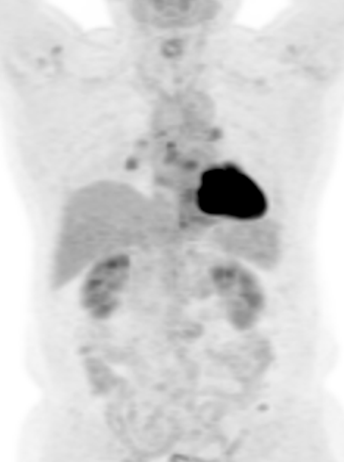
\includegraphics[height=11.8mm]{assets/pet_mip_icon.png}};%
}
\newcommand{\iconclinical}[2]{%
  \begin{scope}[shift={#2}]
    \begin{scope}
      \clip[rounded corners=2.5pt] (-5.25mm,-6mm) rectangle (5.25mm,6mm);
      \fill[boxpurple] (-5.25mm,-6mm) rectangle (5.25mm,6mm);
      \fill[navy!28]   (-5.25mm,3.3mm) rectangle (5.25mm,6mm);
      \draw[navy!45, line width=0.35pt]
        (-5.25mm,3.3mm) -- (5.25mm,3.3mm)  (-5.25mm,0.8mm) -- (5.25mm,0.8mm)
        (-5.25mm,-1.7mm) -- (5.25mm,-1.7mm) (-5.25mm,-4.2mm) -- (5.25mm,-4.2mm)
        (-1.75mm,-6mm) -- (-1.75mm,6mm)     (1.75mm,-6mm) -- (1.75mm,6mm);
    \end{scope}
    \draw[navy, line width=0.7pt, rounded corners=2.5pt] (-5.25mm,-6mm) rectangle (5.25mm,6mm);
    \node[minimum width=10.5mm, minimum height=12mm, inner sep=0pt] (#1) at (0,0) {};
  \end{scope}%
}
\newcommand{\iconreport}[2]{%
  \begin{scope}[shift={#2}]
    \fill[boxpink] (-4.6mm,-6mm) -- (-4.6mm,6mm) -- (1.7mm,6mm) -- (4.6mm,3.1mm) -- (4.6mm,-6mm) -- cycle;
    \draw[navy, line width=0.7pt, rounded corners=1pt]
      (-4.6mm,-6mm) -- (-4.6mm,6mm) -- (1.7mm,6mm) -- (4.6mm,3.1mm) -- (4.6mm,-6mm) -- cycle;
    \fill[navy!20] (1.7mm,6mm) -- (1.7mm,3.1mm) -- (4.6mm,3.1mm) -- cycle;
    \draw[navy, line width=0.55pt] (1.7mm,6mm) -- (1.7mm,3.1mm) -- (4.6mm,3.1mm);
    \draw[navy!55, line width=0.5pt]
      (-2.9mm,1.4mm) -- (2.9mm,1.4mm)  (-2.9mm,-0.4mm) -- (2.9mm,-0.4mm)
      (-2.9mm,-2.2mm) -- (2.9mm,-2.2mm) (-2.9mm,-4.0mm) -- (0.9mm,-4.0mm);
    \node[minimum width=9.2mm, minimum height=12mm, inner sep=0pt] (#1) at (0,0) {};
  \end{scope}%
}

\begin{document}
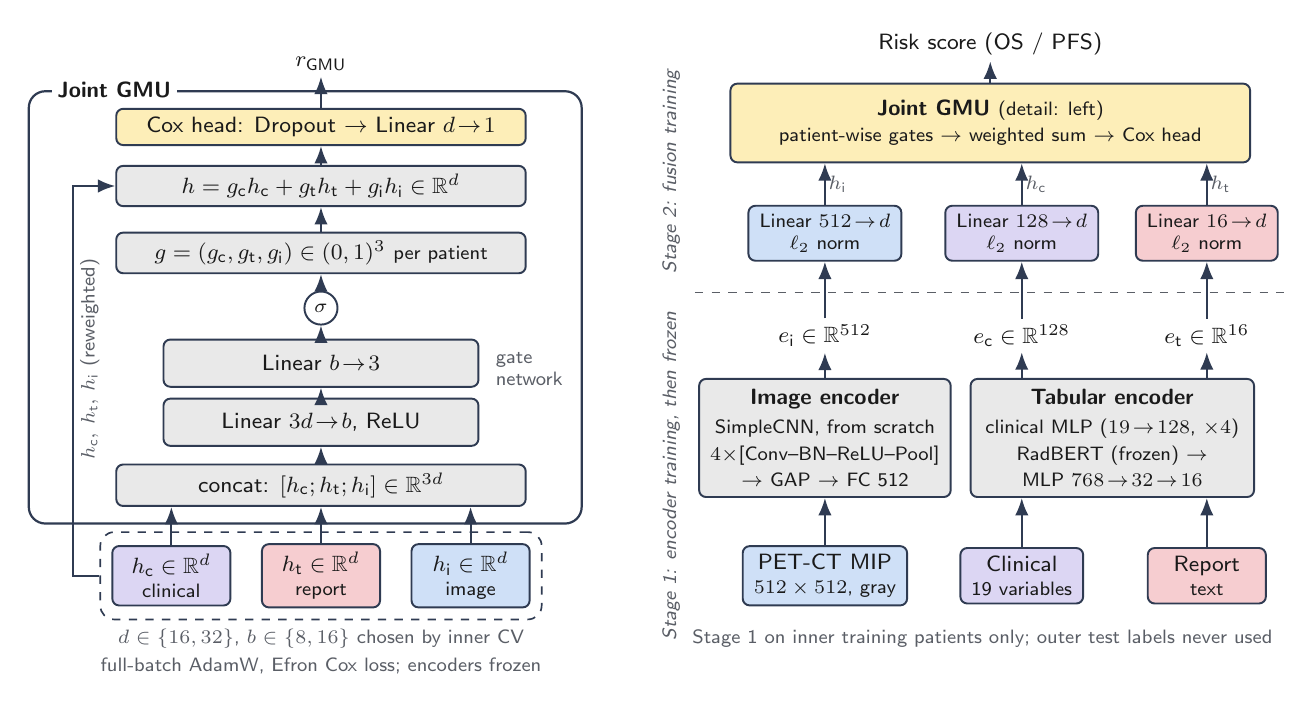
\begin{tikzpicture}[x=1cm,y=1cm]

% ===================== LEFT: Joint GMU (detail) =====================
\begin{scope}[shift={(0,0)}]
  % inputs: projected, l2-normalised features
  \node[inp=boxpurple] (hc) at (0,0)   {$h_{\text{c}}\in\mathbb{R}^{d}$\\[-1pt]{\scriptsize clinical}};
  \node[inp=boxpink]   (ht) at (1.9,0) {$h_{\text{t}}\in\mathbb{R}^{d}$\\[-1pt]{\scriptsize report}};
  \node[inp=boxblue]   (hi) at (3.8,0) {$h_{\text{i}}\in\mathbb{R}^{d}$\\[-1pt]{\scriptsize image}};
  % gate network
  \node[blk, minimum width=52mm] (cat) at (1.9,1.15) {concat: $[h_{\text{c}};h_{\text{t}};h_{\text{i}}]\in\mathbb{R}^{3d}$};
  \node[lay, minimum width=40mm] (g1)  at (1.9,1.95) {Linear $3d\!\to\!b$, ReLU};
  \node[lay, minimum width=40mm] (g2)  at (1.9,2.7)  {Linear $b\!\to\!3$};
  \node[op]                      (sg)  at (1.9,3.4)  {$\sigma$};
  \node[blk, minimum width=52mm] (gv)  at (1.9,4.1)  {$g=(g_{\text{c}},g_{\text{t}},g_{\text{i}})\in(0,1)^3$ {\scriptsize per patient}};
  % weighted sum, Cox head
  \node[blk, minimum width=52mm] (sum) at (1.9,4.95) {$h=g_{\text{c}}h_{\text{c}}+g_{\text{t}}h_{\text{t}}+g_{\text{i}}h_{\text{i}}\in\mathbb{R}^{d}$};
  \node[blk=boxyellow, minimum width=52mm] (hd) at (1.9,5.7) {Cox head: Dropout $\to$ Linear $d\!\to\!1$};
  \node[risk] (r) at (1.9,6.5) {$r_{\text{GMU}}$};
  % arrows
  \draw[arr] (hc) -- (hc |- cat.south);
  \draw[arr] (ht) -- (cat);
  \draw[arr] (hi) -- (hi |- cat.south);
  \draw[arr] (cat) -- (g1);  \draw[arr] (g1) -- (g2);  \draw[arr] (g2) -- (sg);
  \draw[arr] (sg) -- (gv);   \draw[arr] (gv) -- (sum); \draw[arr] (sum) -- (hd);
  \draw[arr] (hd) -- (r);
  % skip path: the same three features are reweighted by the gates
  \begin{scope}[on background layer]
    \node[armbox, fit=(hc)(ht)(hi)] (fg) {};
  \end{scope}
  \draw[arr] (fg.west) -- (-1.25,0) -- (-1.25,4.95) -- (sum.west);
  \node[lab, rotate=90, anchor=north] at (-1.2,2.75) {$h_{\text{c}},\,h_{\text{t}},\,h_{\text{i}}$ (reweighted)};
  % gate-network bracket
  \begin{scope}[on background layer]
    \node[armbox, fit=(g1)(g2)(sg), inner xsep=3pt] (gn) {};
  \end{scope}
  \node[lab, anchor=west, align=left] at ($(gn.east)+(0.05,0)$) {gate\\ network};
  % container
  \begin{scope}[on background layer]
    \node[container, fit={(cat)(gn)(hd)(-1.6,1.15)(5.0,1.15)}] (gmu) {};
  \end{scope}
  \node[font=\footnotesize\bfseries, fill=white, inner sep=2pt, anchor=west]
        at ($(gmu.north west)+(0.3,0)$) {Joint GMU};
  \node[lab] at (1.9,-0.8) {$d\in\{16,32\}$, $b\in\{8,16\}$ chosen by inner CV};
  \node[lab] at (1.9,-1.15) {full-batch AdamW, Efron Cox loss; encoders frozen};
\end{scope}

% ===================== RIGHT: full model =====================
\begin{scope}[shift={(8.3,0)}]
  % inputs
  \node[inp=boxblue]   (im) at (0,0)    {PET-CT MIP\\[-1pt]{\scriptsize $512\times512$, gray}};
  \node[inp=boxpurple] (cl) at (2.5,0) {Clinical\\[-1pt]{\scriptsize 19 variables}};
  \node[inp=boxpink]   (rp) at (4.85,0) {Report\\[-1pt]{\scriptsize text}};
  % encoders (Stage 1)
  \node[blk, minimum width=30mm, minimum height=15mm] (ie) at (0,1.75)
        {\textbf{Image encoder}\\[1pt] {\scriptsize SimpleCNN, from scratch}\\ {\scriptsize $4\times$[Conv--BN--ReLU--Pool]}\\ {\scriptsize $\to$ GAP $\to$ FC 512}};
  \node[blk, minimum width=36mm, minimum height=15mm] (te) at (3.65,1.75)
        {\textbf{Tabular encoder}\\[1pt] {\scriptsize clinical MLP ($19\!\to\!128$, $\times4$)}\\ {\scriptsize RadBERT (frozen) $\to$}\\ {\scriptsize MLP $768\!\to\!32\!\to\!16$}};
  % encoder features
  \node[risk] (ei) at (0,3.05)    {$e_{\text{i}}\in\mathbb{R}^{512}$};
  \node[risk] (ec) at (2.5,3.05) {$e_{\text{c}}\in\mathbb{R}^{128}$};
  \node[risk] (et) at (4.85,3.05) {$e_{\text{t}}\in\mathbb{R}^{16}$};
  % Stage separator
  \draw[dashed, ink2, line width=0.4pt] (-1.65,3.6) -- (5.85,3.6);
  \node[stage, rotate=90, anchor=east] at (-1.95,3.4)  {Stage 1: encoder training, then frozen};
  \node[stage, rotate=90, anchor=west] at (-1.95,3.8) {Stage 2: fusion training};
  % projections (Stage 2)
  \node[blk=boxblue,   minimum width=17mm, font=\scriptsize] (pi) at (0,4.35)    {Linear $512\!\to\!d$\\ $\ell_2$ norm};
  \node[blk=boxpurple, minimum width=17mm, font=\scriptsize] (pc) at (2.5,4.35) {Linear $128\!\to\!d$\\ $\ell_2$ norm};
  \node[blk=boxpink,   minimum width=17mm, font=\scriptsize] (pt) at (4.85,4.35) {Linear $16\!\to\!d$\\ $\ell_2$ norm};
  % GMU
  \node[blk=boxyellow, minimum width=66mm, minimum height=10mm] (gm) at (2.1,5.75)
        {\textbf{Joint GMU} {\scriptsize(detail: left)}\\ {\scriptsize patient-wise gates $\to$ weighted sum $\to$ Cox head}};
  \node[risk] (out) at (2.1,6.75) {Risk score (OS / PFS)};
  % arrows
  \draw[arr] (im) -- (ie);  \draw[arr] (cl) -- (cl |- te.south);  \draw[arr] (rp) -- (rp |- te.south);
  \draw[arr] (ie) -- (ei);
  \draw[arr] (cl |- te.north) -- (ec);
  \draw[arr] (rp |- te.north) -- (et);
  \draw[arr] (ei) -- (pi);  \draw[arr] (ec) -- (pc);  \draw[arr] (et) -- (pt);
  \draw[arr] (pi.north) -- node[lab, right] {$h_{\text{i}}$} (pi.north |- gm.south);
  \draw[arr] (pc.north) -- node[lab, right] {$h_{\text{c}}$} (pc.north |- gm.south);
  \draw[arr] (pt.north) -- node[lab, right] {$h_{\text{t}}$} (pt.north |- gm.south);
  \draw[arr] (gm) -- (out);
  \node[lab] at (2.0,-0.8) {Stage 1 on inner training patients only; outer test labels never used};
\end{scope}

\end{tikzpicture}
\end{document}
